\documentclass[12pt]{article}

\usepackage[margin=0.8 in]{geometry}
\usepackage{amsmath}
\usepackage{amssymb}
\usepackage{mathtools}
\usepackage{enumerate}
\usepackage{verbatim}
\usepackage{amsthm}
\usepackage{hyperref}

\title{}
%\content{}



\let \proj \undefined
\newcommand{\p}{\partial}
\newcommand{\R}{ \mathbb{R}}

\DeclareMathOperator{\proj}{proj}
\newcommand{\sS}{\mathscr{S}}
\DeclareMathOperator{\comp}{comp}
\newcommand{\A}{\mathcal{A}}
\newcommand{\D}{\mathcal{D}}
\newcommand{\e}{\epsilon}
\newcommand{\et}{\tilde{\e}}
\newcommand{\vr}{\vec{r}{}}
\newcommand{\vF}{\vec{F}}
\newcommand{\triple}{\iiint_E f(x,y,z)dV}
\renewcommand{\lg}{\langle}
\newcommand{\rg}{\rangle}
\newcommand{\Q}{\frac{\p Q}{\p x}}
\renewcommand{\P}{\frac{\p P}{\p y}}
\let\implies\Rightarrow
\newcommand{\n}{\nabla}
\newcommand{\Fline}{\vF\cdot d\vr}
\newcommand{\vi}{\vec{i}}
\newcommand{\vj}{\vec{j}}
\newcommand{\vk}{\vec{k}}
\DeclareMathOperator{\curl}{curl}
%\newcommand{\n}{\nabla}




\newenvironment{solution}
  {\begin{proof}[Solution]}
  {\end{proof}
  
  }
\newtheorem{example}{Example}
\newtheorem{exercise}{Exercise}
\newtheorem{theorem}{Theorem}
\newtheorem{defn}{Definition}
\newcommand{\rcross}{\vr_u\times\vr_v} 




\begin{document}
\section*{Orientations}
The goal of the last few sections of Math 324 is to make sense of integrals on surfaces and state some results about them. Recall from a previous section that when we talked about line integrals, some of them depended on the parameterization of the curve, and more specifically on the direction the curve was transversed, whereas others didn't. It's therefore natural to expect that we might have to deal with some similar behavior when discussing surface integrals.

%\section*{Orientations }
The surface analogue of choosing a ``direction'' is called a choice of orientation, and is essentially a choice of a preferred side of a surface. For example, we might want to consider the interior or the exterior of a sphere to be its preferred side.

Note that choosing a preferred side might not be possible for some surfaces. The mathematicians' favorite such surface is called a M{\"o}bius strip, a surface that has only one side.

In Math 324 we will only deal with orientable surfaces.

\begin{itemize}
\item A nice animation on  M{\"o}bius strip, \href{https://www.youtube.com/watch?v=XlQOipIVFPk}{here}.
\item A video explaining the proper way to cut a bagel, along a M{\"o}bius strip, \href{https://www.youtube.com/watch?v=Ktfo8D3cCr0}{here}.
\end{itemize}

\begin{defn}
The surfaces for which we can choose an orientation (preferred side) are called \textbf{orientable}.
\end{defn}


More rigorously, orientations are described in terms of unit normal vector fields. At each point of a parametric surface that is sufficiently regular (i.e. has no cusps) we can find 2 vectors that have unit length and are normal to the tangent plane of the surface at the given point. By choosing one of them at each point, we can form a vector field on the surface (since we are making sense of a function that takes points on the surface as input and outputs vectors). Now we want to choose a unit normal vector at each point so that our vector field becomes continuous (for example, in a sphere we should choose vectors pointing only inwards or only outwards)
\begin{defn}
An orientation on an orientable surface is a choice of a continuous unit normal vector field. 
\end{defn}


\begin{figure}[h]
\minipage{0.32\textwidth}
  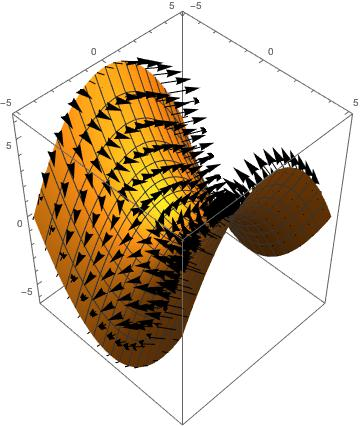
\includegraphics[width=\linewidth]{t2.jpeg}
  \caption{Elliptic Paraboloid, with upward pointing unit normal vector field.}\label{fig3}
\endminipage\hfill
\minipage{0.32\textwidth}
  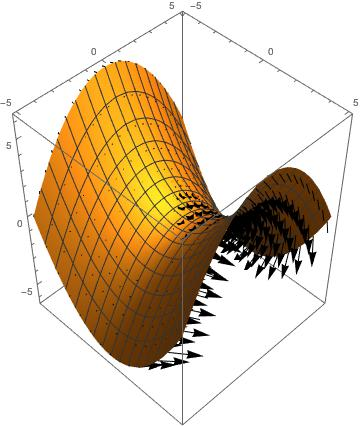
\includegraphics[width=\linewidth]{t3.jpeg}
  \caption{Elliptic Paraboloid, with downward pointing unit normal vector field.}\label{fig4}
\endminipage\hfill
\minipage{0.32\textwidth}%
  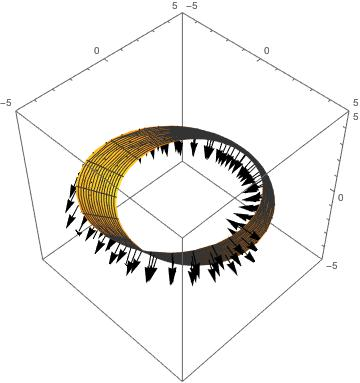
\includegraphics[width=\linewidth]{t1.jpeg}
  \caption{A M{\"o}bius strip, where it's not possible to choose a continuous unit normal vector field.}\label{fig5}
\endminipage
\end{figure}


\subsection*{In Practice:} 
How can we find a unit normal vector field for a given orientable parametric surface? From a parametrization $\vr(u,v)$ we can automatically find 2 continuous unit vector fields, as discussed in the previous section, namely $$\frac{\rcross(u,v)}{|\rcross(u,v)|}$$ and 
$$-\frac{\rcross(u,v)}{|\rcross(u,v)|}.$$
Usually, a problem will tell us which orientation we are expected to use, using expressions described on page 2.
 So: \begin{itemize}
 \item We compute one of the unit normal vector fields to the surface ($\frac{\rcross(u,v)}{|\rcross(u,v)|}$ or $-\frac{\rcross(u,v)}{|\rcross(u,v)|}$). 
 \item We pick a point on the surface* and check if the normal vector given by our vector field agrees with the orientation given by the problem.
\item If yes, we work with our vector field, otherwise we work we use its negative.
 \end{itemize}

*As a guideline for picking a point to check on a parametrized surface, it is better to avoid choosing points on the image of the boundary of the domain $D$ where the parametrization is defined. For example, in a sphere parametrized as $$\vr(u,v)=\lg R\sin(u)\cos(v),R\sin(u)\cos(v),R\cos(u)\rg, (u,v)\in [0,\pi]\times [0,2\pi]$$ it is safer to not choose points that correspond to $u=0, u=\pi$, $v=0$, $v=2\pi$. As we found in the previous section, $|\rcross(u,v)|=R^2\sin(u)$ for and this parametrization and therefore $\vr(u,v)=\vec{0}$ whenever $u=0$ or $u=\pi$, which doesn't help us decide on the correct orientation. It would be safer to choose, for example, $u=v=\frac{\pi}{4}$. 

\subsection*{Some common expressions}
Some expressions you might come across while doing problems are the following:
\begin{itemize}
\item \textbf{Outward/Inward orientation:} This applies for \textbf{closed } surfaces, that is, surfaces that are the boundary of a domain in $\R^3$, such as a sphere or an ellipsoid. Such surfaces split $\R^3$ into a bounded and an unbounded domain. Then, outward orientation means that the unit normal vector field we choose is pointing towards the unbounded domain, and the opposite for inward orientation. Outward/inward orientation can be referred to as \textbf{positive/negative} orientation, respectively.
\item \textbf{Upward/downward orientation:} It means that the $z$ coordinate of $\frac{\rcross(u,v)}{|\rcross(u,v)|}$ is positive/negative respectively, for all $(u,v)$.
\item\textbf{ In the direction of the positive $x/y/z$ axis: } It means that the $x/y/z$ coordinate of $\frac{\rcross(u,v)}{|\rcross(u,v)|}$ respectively is positive , for all $(u,v)$.
\end{itemize}

\subsection*{Examples}

\begin{example}
Decide if the orientation given by $\frac{\rcross(u,v)}{|\rcross(u,v)|}$ is upward on downward, where $\vr(u,v)=\lg u,v, f(u,v)\rg$, $(u,v)\in D$ and $f$ is a differentiable function.
\end{example}
\begin{solution}
We have $$\rcross(u,v)=\lg -\frac{\p f}{\p u}, -\frac{\p f}{\p v},1\rg$$
so 
$$\frac{\rcross(u,v)}{|\rcross(u,v)|}=\dfrac{\lg -\frac{\p f}{\p u}, -\frac{\p f}{\p v},1\rg}{\sqrt{\left (\frac{\p f}{\p u}\right )^2+\left (\frac{\p f}{\p v}\right )^2+1}}$$
and the $z$ coordinate is $$\frac{1}{\sqrt{\left (\frac{\p f}{\p u}\right )^2+\left (\frac{\p f}{\p v}\right )^2+1}}>0,$$ so the orientation is upward.

\end{solution}


\begin{example}
Decide if the orientation given by $\frac{\rcross(u,v)}{|\rcross(u,v)|}$ is outward on inward, where $$\vr(u,v)=\lg \sin(u)\cos(v),\sin(u)\sin(v),\cos(u)\rg,\text{ for }(u,v)\in[0,\pi]\times[0,2\pi]$$ is the usual parametrization for the unit sphere.
\end{example}

\begin{solution}
As in the previous section, we find $$\rcross(u,v)=\lg\sin^2(u)\cos(v),\sin^2(u)\sin(v),\cos^2(v)\cos(u)\sin(u)+\sin^2(v)\cos(u)\sin(u)\rg$$
and $$|\rcross(u,v)|=\sin(u),$$ so 
$$\frac{\rcross(u,v)}{|\rcross(u,v)|}=\lg\sin(u)\cos(v),\sin(u)\sin(v),\cos(u)\rg.$$
Choosing, for example, $u=\frac{\pi}{2}$, $v=\frac{\pi}{2}$ we find the vector $\lg 0,1,0\rg$ mounted on the point $(0,1,0)$. Drawing a picture, we see that the vector field has to be outward pointing.
\begin{figure}[h]
\begin{center}
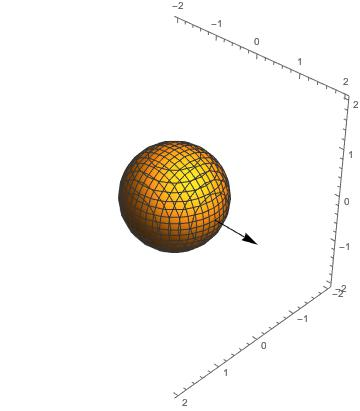
\includegraphics[scale=.3]{out.jpeg}
\end{center}
\end{figure}
\end{solution}
\end{document}

